% -*- LaTeX -*-
% -*- coding: utf-8 -*-
%
% ~~~~~~~~~~~~~~~~~~~~~~~~~~~~~~~~~~~~~~~~~~~~~~~~~~~~~~~~~~~~~~~~~~~~~~~~~~~~~~
%
%                             michael a.g. aïvázis
%                      california institute of technology
%                      (c) 1998-2010  all rights reserved
%
% ~~~~~~~~~~~~~~~~~~~~~~~~~~~~~~~~~~~~~~~~~~~~~~~~~~~~~~~~~~~~~~~~~~~~~~~~~~~~~~
%

\lecture{Matrices}{20100303}

% --------------------------------------
% contact detection
\begin{frame}[fragile]
%
  \frametitle{Dense matrix problems}
%
  \begin{itemize}
%
  \item we'll take a look at
    \begin{itemize}
    \item inner and outer products of two vector
    \item matrix-vector and matrix-matrix multiplication
    \item $LU$ factorization and Cholesky decomposition
    \item QR factorization
    \item computing eigenvalues and eigenvectors
    \item fast Fourier transforms
    \end{itemize}
%
  \item when solving a problem of size $n$ on $p$ processors, we will assume
    \begin{itemize}
    \item that $p$, and occasionally $\sqrt{p}$ divides $n$
    \item that $p$ is a perfect square, when forming two-dimensional process grids
    \item matrices are $n\times n$ -- square, not rectangular
    \item we are memory constrained and data replication must be minimized
    \end{itemize}
%
    \item these problems have been studied extensively and form the core of scientific
      computing on parallel machines
      \begin{itemize}
      \item excellent implementations available 
      \item interest has been revived due to the expected disruption by multi-core
        architectures
      \end{itemize}
%
  \end{itemize}
%
\end{frame}

% --------------------------------------
% vector inner product
\begin{frame}[fragile]
%
  \frametitle{Vector inner product}
%
  \begin{itemize}
%
  \item the inner product of two $n$-vectors $x$, $y$ is given by
    \begin{equation}
    x^{T}y = \sum_{i=1}^{n} x_{i}y_{i}
    \end{equation}
    which requires $n$ multiplications and $n-1$ additions
%
  \item parallelization strategy:
    \begin{itemize}
    \item $n$ fine grain tasks, numbered $i = 1, \ldots, n$, that store $x_{i}$ and $y_{i}$,
      and compute $x_{i} y_{i}$
    \item communication is a sum reduction over $n$ fine grain tasks
    \item coarsening is achieved by coalescing $n/p$ tasks together, assuming that each process
      can accommodate the data storage requirements
    \item and mapping each coarse grain task to a process
    \end{itemize}
%
  \end{itemize}
%
\end{frame}

% --------------------------------------
% vector outer product
\begin{frame}[fragile]
%
  \frametitle{Vector outer product}
%
  \begin{itemize}
%
  \item the outer product of two $n$-vectors $x$ and $y$ is the $n \times n$ matrix $A$ given
    by
    \begin{equation}
      A_{ij} = x_{i} y_{j}
    \end{equation}
    which requires $n^{2}$ multiplications
%
  \item parallelization strategies are determined by the storage requirements
    \begin{itemize}
    \item build a two-dimensional grid of $n^{2}$ fine grain tasks numbered $(i,j)$, with $i,j
      = 1, \ldots, n$; each one computes $x_{i}y_{j}$
    \item assuming no data replication is allowed
      \begin{itemize}
      \item let task $(i,1)$ store $x_{i}$ and task $(1,i)$ store $y_{i}$
      \item or, let task $(i,i)$ store both $x_{i}$ and $y_{i}$
      \end{itemize}
    \item either way, the task that owns each element must broadcast it to the other tasks:
      $x_{i}$ along the \th{i} task row, $y_{j}$ along the \th{j} task column
    \item coarsening to $p$ tasks can be accomplished by
      \begin{itemize}
      \item combining $n/p$ rows or columns
      \item forming $(n/\sqrt{p}) \times (n/\sqrt{p})$ grid of fine grain tasks
      \end{itemize}
    \item and each coarse grain task can be assigned to a process
    \end{itemize}
%
  \item either way, na\"ive broadcasting of the components of $x$ and $y$ would require as much
    total memory as replication
    \begin{itemize}
    \item storage can be reduced by circulating portions of $x$ and $y$ through the tasks, with
      each task using the available portion and passing it on
    \end{itemize}
%
  \end{itemize}
%
\end{frame}

% --------------------------------------
% matrix vector product
\begin{frame}[fragile]
%
  \frametitle{The product of a matrix with a vector}
%
  \begin{itemize}
%
  \item given an $n \times n$ matrix $A$ and an $n$-vector $x$, the matrix vector product
    yields an $n$-vector $y$ whose components are given by
    \begin{equation}
      y_{i} = \sum_{j=1}^{n} A_{ij} x_{j}
    \end{equation}
    requiring a total of $n^{2}$ multiply-add operations
%
  \item once again, the parallelization strategy is determined by how the data is distributed
    among fine grain tasks
    \begin{itemize}
    \item build a two-dimensional grid of $n^{2}$ fine grain tasks numbered $(i,j)$, with $i,j
      = 1, \ldots, n$; each one computes $A_{ij}x_{j}$
    \item task $(i,j)$ has $A_{i,j}$, but if no data replication is allowed
      \begin{itemize}
      \item let task $(i,1)$ store $x_{i}$ and task $(1,i)$ store $y_{i}$
      \item or, let task $(i,i)$ store both $x_{i}$ and $y_{i}$
      \end{itemize}
    \item the task that owns $x_{j}$ must broadcast it along the \th{j} task row, and $y_{i}$
      is formed by sum reduction along the \th{i} task column
    \item coarsening into $p$ tasks can be accomplished by combining $n/p$ rows/columns, or by
      forming $(n/\sqrt{p}) \times (n/\sqrt{p})$ blocks
    \item and each coarse grain task can be assigned to a process
    \end{itemize}
%
  \end{itemize}
%
\end{frame}

% --------------------------------------
% coarsening matrix vector product
\begin{frame}[fragile]
%
  \frametitle{Coarsening along rows or columns}
%
  \begin{itemize}
%
  \item for one-dimensional coarsening into $n/p$ task rows
    \begin{itemize}
    \item if $x$ is stored in one task, it must be broadcast to all others
    \item if $x$ is distributed among tasks, with $n/p$ components per task, then multiple
      broadcasts are required
    \item each task computes the inner product of its $n/p$ rows of $A$ with the entire $x$ to
      produce $n/p$ components of $y$
    \end{itemize}
%
  \item for one-dimensional coarsening into $n/p$ task columns
    \begin{itemize}
    \item $n/p$ components of $x$ are distributed among the tasks
    \item each task computes the linear combination of its $n/p$ columns with coefficients
      from its copy of $x$
    \item since the right parts of $x$ are already available, no communication is required
    \item $y$ is generated by a sum reduction across tasks
    \end{itemize}
%
  \item these two are {\em duals} of each other
    \begin{itemize}
    \item row coarsening begins with broadcast, followed by communication-free inner products
    \item column coarsening begins with communication-free linear combinations, follows by a
      reduction
    \end{itemize}
%
  \end{itemize}
%
\end{frame}

% --------------------------------------
% 2d coarsening
\begin{frame}[fragile]
%
  \frametitle{Two dimensional coarsening}
%
  \begin{itemize}
%
  \item for two dimensional coarsening, we form $(n/\sqrt{p}) \times (n/\sqrt{p})$ blocks of
    fine grain task
    \begin{itemize}
    \item each one holding a $(n/\sqrt{p}) \times (n/\sqrt{p})$ block of $A$
    \item with components of $x$ distributed either across one task row, or along the diagonal,
      $n/p$ components per task
    \end{itemize}
%
  \item the algorithm combines the features of row/column coarsening
    \begin{itemize}
    \item components of $x$ are broadcast along task columns
    \item each task performs $n^{2}/p$ multiplications locally and sums $n/\sqrt{p}$ sets of
      products
      \item sum reductions along task rows produce the components of $y$ by combining the
        component products
    \end{itemize}
%
  \end{itemize}
%
\end{frame}

% --------------------------------------
% matrix-matrix multiply
\begin{frame}[fragile]
%
  \frametitle{Matrix multiplication}
%
  \begin{itemize}
%
  \item the product of two $n \times n$ matrices $A$ and $B$ is an $n \times n$ matrix $C$
    given by
    \begin{equation}
      C_{ij} = \sum_{k=1}^{n} A_{ik} B_{kj}
    \end{equation}
    where each one of $n^{2}$ entries requires $n$ multiply-adds for a total of $n^{3}$
    operations
%
  \item matrix multiplication can be viewed as
    \begin{itemize}
    \item $n^{2}$ inner products
    \item the sum of $n$ outer products
    \item $n$ matrix vector products
    \end{itemize}
%
  \item each one produces a parallel algorithm for matrix multiplication
%
  \item but we'll explore a direct solution instead
%
  \end{itemize}
%
\end{frame}

% --------------------------------------
% matrix-matrix multiply: partitioning and communication
\begin{frame}[fragile]
%
  \frametitle{Partitioning and communication patterns}
%
  \begin{itemize}
%
  \item we build a three dimensional array of $n^{3}$ fine grain tasks
    \begin{itemize}
    \item with $i,j,k = 1,\ldots,n$, let task $(i,j,k)$ be responsible for computing the
      product $A_{ij}B_{jk}$
    \item assuming no data replication, we have to distribute the data for $A$ and $B$ among
      $2n^{2}$ tasks
    \item suppose that task $(i,j,j)$ holds $A_{i,j}$ and task $(i,j,i)$ holds $B_{i,j}$
    \item we will refer to tasks along $i$ and $j$ as task rows and columns
    \item and tasks along $k$ as {\em layers}
    \end{itemize}
%
  \item the communication requirements among tasks are satisfied if we
    \begin{itemize}
    \item broadcast the entries of the \th{k} column of $A$ from task $(i,j,j)$ to each task
      row in the \th{k} layer
    \item broadcast the entries of the \th{k} row of $B$ from task $(i,j,i)$ to each task column of
      the \th{k} layer
    \item form the result $C_{ij}$ by the sum reduction of the values held by all the
      tasks layers $k$
    \end{itemize}
%
  \end{itemize}
%
\end{frame}

% --------------------------------------
% coarsening
\begin{frame}[fragile]
%
  \frametitle{Coarsening}
%
  \begin{itemize}
%
  \item there are four natural ways to coarsen our $n \times n \times n$ fine grain tasks into
    $p$ coarse grain tasks
    \begin{itemize}
    \item by task rows: combine the $(n/p) \times n \times n$ tasks along a given task row
    \item by task columns: combine the $n \times (n/p) \times n$ tasks along a given task
      column
    \item partition the layers in a two dimensional grid by combining $(n/\sqrt{p}) \times
      (n/\sqrt{p}) \times n$ fine grain tasks
    \item using three dimensional blocks by combining $(n/\sqrt[3]{p}) \times (n/\sqrt[3]{p})
      \times (n/\sqrt[3]{p})$ tasks
    \end{itemize}
%
    \item the two one dimensional coarsening strategies are similar
      \begin{itemize}
      \item for row coarsening
        \begin{itemize}
        \item each task needs only the part of $A$ it already has, but needs all $B$ entries
        \item so global communication is required to broadcast the $n^{2}/p$ entries of $B$ held
          by each task
        \end{itemize}
      \item conversely, for column coarsening
        \begin{itemize}
        \item each task needs only the parts of $B$ that it already has, but it needs all of $A$
        \item so global communication is required to broadcast the $n^{2}/p$ entries of $A$ held
          by each task
        \end{itemize}
      \item if accumulating $A$ or $B$ on each processor is not feasible, tasks can circulate
        portions of the array in a ring
%
      \end{itemize}
%
  \end{itemize}
%
\end{frame}

% --------------------------------------
% 2d coarsening
\begin{frame}[fragile]
%
  \frametitle{Coarsening using a two dimensional grid}
%
  \begin{itemize}
%
  \item block matrix multiplication has the same overall form as actual product, with scalar
    operations replaced by the matrix product of blocks!
%
  \item you should verify that
    \begin{equation}
      C_{ij} = \sum_{k=1}^{\sqrt{p}} A_{ik} B_{kj}
    \end{equation}
    for $i,j = 1, \ldots, \sqrt{p}$
%
  \item assume that task $(i,j$) has local access to block $A_{ij}$ and $B_{ij}$ and computes
    block $C_{ij}$ of the result
%
  \item this requires all blocks $A_{ik}$ and $B_{kj}$ for $k=1,\ldots,\sqrt{p}$ to be
    communicated
    \begin{itemize}
    \item first, a global broadcast of $A$ blocks across each task row 
    \item followed by a global broadcast of $B$ blocks across each task column 
    \end{itemize}
%
  \item memory requirements can be addressed by either of the following:
    \begin{itemize}
    \item broadcast blocks of $A$ across rows while circulating blocks of $B$ across columns in
      lock step, so that they arrive at a given task at the same time
    \item circulate blocks of $A$ horizontally and blocks of $B$ vertically, after an initial
      circular shift, so that blocks meet at a given task at the right time
    \end{itemize}
%
  \end{itemize}
%
\end{frame}

% --------------------------------------
% LU factorization
\begin{frame}[fragile]
%
  \frametitle{$LU$ factorization}
%
  \begin{itemize}
%
  \item systems of linear equations are ubiquitous in numerical analysis
  \item let $A$ be an $n \times n$ matrix, $b$ a known $n$-vector; we are looking for $x$ such
    that
    \begin{equation}
      A x = b \label{eq:linear-system}
    \end{equation}
  \item a commonly used direct method for solving this system is to convert $A$ into the
    product of a lower triangular matrix $L$ with an upper triangular matrix $U$
    \begin{equation}
      A = L U \label{eq:LU-factorization}
    \end{equation}
    known as $LU$ factorization
  \item \eqref{linear-system} becomes
    \begin{equation}
      L U x = b
    \end{equation}
    which we can now solve in two simpler steps
    \begin{eqnarray}
        L y & = & b \\
        U x & = & y
    \end{eqnarray}
    where we first solve the lower triangular system by forward substitution, followed by
    solving the upper triangular system by back substitution to obtain $x$
%
  \end{itemize}
%
\end{frame}

% --------------------------------------
% LU by Gaussian elimination
\begin{frame}[fragile]
%
  \frametitle{$LU$ by Gaussian elimination}
%
  \begin{itemize}
%
  \item we can compute the $LU$ factorization of $A$ using Gaussian elimination
    \begin{center}
      \begin{minipage}{.85\linewidth}
        \begin{algorithm}[H]
          \label{alg:LU-gaussian}
%
          \dontprintsemicolon
          % \nocaptionofalgo
          \setalcaphskip{0ex}
%
          \caption{\lu(A)}
%
          \For{$k=1$ \KwTo $n-1$}{
            \For{$i=k+1$ \KwTo $n$}{
              $L_{ik} = A_{ik} / A_{kk}$
            }
            \For{$j=k+1$ \KwTo $n$}{
              \For{$i=k+1$ \KwTo $n$}{
                $A_{ij} = A_{ij} - L_{ik}A_{kj}$
              }
            }
          }
%
        \end{algorithm}
      \end{minipage}
    \end{center}
%
    which encodes $L$ and $U$ in place by overwriting $A$
%
  \item \algref{LU-gaussian} requires roughly $n^{3}/3$ multiply-adds and $n^{2}/2$ divisions
%
  \item we may also need {\em pivoting} to ensure numerical stability (and existence)
%
  \item \algref{LU-gaussian} is one of many algorithms expressed essentially as a triply nested loop
    \begin{itemize}
    \item the three indices can be ordered in any of $3!$ ways, with totally different memory
      access patterns
    \item in parallel, the $kij$ and $kji$ forms may be the most efficient
    \end{itemize}
%
  \end{itemize}
%
\end{frame}
%

% --------------------------------------
% parallelization strategy
\begin{frame}[fragile]
%
  \frametitle{Parallel $LU$ decomposition}
%
  \begin{itemize}
%
  \item number fine grain tasks as $(i,j)$ with $i,j = 1, \ldots, n$; each task
    \begin{itemize}
    \item stores $A_{ij}$
    \item computes and stores $U_{ij}$, if $i \leq j$
    \item computes and stores $L_{ij}$, if $i > j$
    \end{itemize}
    yielding a two dimensional array of $n^{2}$ tasks
%
  \item no need to compute and store
    \begin{itemize}
    \item the zeroes in the lower triangle of $U$
    \item the unit diagonal and the zeroes in the upper triangle of $L$
    \end{itemize}
%
  \item in order to create $p$ coarse grain tasks we could combine
    \begin{itemize}
    \item $n/p$ rows or columns of fine grain tasks
    \item $(n/\sqrt{p}) \times (n/\sqrt{p})$ blocks of tasks
    \end{itemize}
    and map each one to a process
%
  \end{itemize}
% 
\end{frame}

% --------------------------------------
% parallelization LU
\begin{frame}[fragile]
%
  \frametitle{Communication patterns for parallel $LU$ decomposition}
%
  \begin{center}
    \begin{minipage}{.85\linewidth}
      \begin{algorithm}[H]
        \label{alg:pLU-ij}
%
        \dontprintsemicolon
        % \nocaptionofalgo
        \setalcaphskip{0ex}
%
        \caption{\lu($A$, task=$(i,j)$)}
%
        \For{$k=1$ \KwTo $\min(i,j) - 1$}{
          \KwRecv $A_{kj}$ \;
          \KwRecv $L_{ik}$ \;
          $A_{ij} = A_{ij}- L_{ik}A_{kj}$
        }
        \If{ $i \leq j$}{
          \KwBcast $A_{ij}$ \KwTo $(k,j)$, $k=i+1,\ldots,n$
        } \Else {
          \KwRecv $A_{jj}$ \;
          $L_{ij} = A_{ij}/A_{jj}$ \;
          \KwBcast $L_{ij}$ \KwTo $(i,k)$, $k=i+1,\ldots,n$
        }
% 
      \end{algorithm}
    \end{minipage}
  \end{center}
%
\end{frame}

% --------------------------------------
% row coarsening
\begin{frame}[fragile]
%
  \frametitle{Row coarsening}
%
  \begin{itemize}
%
  \item with one dimensional row coarsening
    \begin{itemize}
    \item we forgo parallelism in updating rows
    \item there is no need to broadcast the multipliers $L_{ij}$ since each row is contained
      entirely within a task
    \item we still need the vertical broadcasts of matrix rows to the tasks below
    \end{itemize}
%
  \end{itemize}
%
  \begin{center}
    \begin{minipage}{.85\linewidth}
      \begin{algorithm}[H]
        \label{alg:pLU-ij-rows}
%
        \dontprintsemicolon
        % \nocaptionofalgo
        \setalcaphskip{0ex}
%
        \caption{\lu($A$, task=$(i,j)$) by rows}
%
        \For{$k=1$ \KwTo $n - 1$}{
          \If{ $k \in myrows$}{
            \KwBcast $\left\{A_{kj} : k\leq j  \leq n\right\}$
          } \Else {
            \KwRecv $\left\{A_{kj} : k\leq j  \leq n\right\}$
          }
          \For{$i \in myrows$, $i > k$} {
            $L_{ik} = A_{ik}/ A_{kk}$
          }
          \For{$j=k+1$ \KwTo $n$}{
            \For{ $i \in myrows$, $i>k$}{
              $A_{ij} = A_{ij} - L_{ik} A_{kj}$
            }
          }
        }
% 
      \end{algorithm}
    \end{minipage}
  \end{center}
% 
\end{frame}

% --------------------------------------
% observations
\begin{frame}[fragile]
%
  \frametitle{Observations on row coarsening}
%
  \begin{itemize}
%
  \item each task becomes idle as soon as it last row is completed
    \begin{itemize}
    \item if rows are contiguous, a task may finish long before the overall computation is done
    \item even worse, updating rows requires progressively less work with increasing row number
    \end{itemize}
%
  \item we may improve concurrency and load balance 
    \begin{itemize}
    \item by assigning rows to tasks in a cyclic manner where row $i$ is updated by task $i
      \mod p$
    \item other mappings may be useful
    \end{itemize}
%
  \item other improvements involve overlapping computation with communication
    \begin{itemize}
    \item at step $k$, each task completes updating its portion of the remaining unreduced
      matrix before moving on to step $k+1$
    \item however, the task that owns the $k+1$ row could broadcast it as soon as it becomes
      available, before moving on to the step $k$ update
    \item this {\em send ahead} strategy may grant other tasks earlier access to the data
      necessary to start working on the next step
    \end{itemize}
%
  \end{itemize}
%
\end{frame}

% --------------------------------------
% column coarsening
\begin{frame}[fragile]
%
  \frametitle{Column coarsening}
%
  \begin{center}
    \begin{minipage}{.85\linewidth}
      \begin{algorithm}[H]
        \label{alg:pLU-ij-columns}
%
        \dontprintsemicolon
        % \nocaptionofalgo
        \setalcaphskip{0ex}
%
        \caption{\lu($A$, task=$(i,j)$) by columns}
%
        \For{$k=1$ \KwTo $n - 1$}{
          \If{ $k \in mycolumns$}{
            \For{ $i=k+1$ \KwTo $n$}{
              $L_{ik} = A_{ik}/ A_{kk}$
            }
            \KwBcast $\left\{L_{ik} : k < i  \leq n\right\}$
          } \Else {
            \KwRecv $\left\{L_{ik} : k < i  \leq n\right\}$
          }
          \For{$i \in mycolumns$, $j > k$} {
            \For{$i=k+1$ \KwTo $n$}{
              $A_{ij} = A_{ij} - L_{ik} A_{kj}$
            }
          }
        }
% 
      \end{algorithm}
    \end{minipage}
  \end{center}
%
  \begin{itemize}
  \item observations similar to row coarsening apply
  \end{itemize}
% 
\end{frame}

% --------------------------------------
% column coarsening
\begin{frame}[fragile]
%
  \frametitle{Block coarsening}
%
  \begin{center}
      \begin{algorithm}[H]
        \label{alg:pLU-ij-blocks}
%
        \dontprintsemicolon
        % \nocaptionofalgo
        \setalcaphskip{0ex}
%
        \caption{\lu($A$, task=$(i,j)$) by blocks}
%
        \For{$k=1$ \KwTo $n - 1$}{
          \If{$k \in myrows$}{
            \KwBcast $\left\{A_{kj} : j \in mycolumns, j>k\right\}$ \KwTo 
            all tasks in my task column
          } \Else {
            \KwRecv $\left\{A_{kj} : j \in mycolumns, j>k\right\}$
          }
          \If{$k \in mycolumns$}{
            \For{$i \in myrows$, $i>k$}{
              $L_{ik} = A_{ik} / A_{kk}$
            }
            \KwBcast $\left\{L_{ik} : i \in myrows, i>k\right\}$ \KwTo 
            all tasks in my task row
          } \Else {
            \KwRecv $\left\{L_{ik} : i \in myrows, i>k\right\}$
          }
          \For{$j \in mycolumns$, $j>k$}{
            \For{$i \in myrows$, $i>k$} {
              $A+{ij} = A_{ij} - L_{ik}A_{kj}$
            }
          }
        }
% 
      \end{algorithm}
  \end{center}
%
\end{frame}

% --------------------------------------
% observations
\begin{frame}[fragile]
%
  \frametitle{Observations on block coarsening}
%
  \begin{itemize}
%
  \item each task becomes idle as soon as it last row and column are completed
    \begin{itemize}
    \item if rows and columns are in contiguous blocks, a task may finish long before the
      overall computation is done
    \item even worse, computing multipliers and updating blocks requires progressively less
      work with increasing row and column numbers
    \end{itemize}
%
  \item we may improve concurrency and load balance 
    \begin{itemize}
    \item by assigning rows and columns to tasks in a cyclic manner where $A_{ij}$ is assigned
      to task $(i \mod \sqrt{p}, j \mod \sqrt{p}$
    \item other mappings may be useful
    \end{itemize}
%
  \item other improvements involve overlapping computation with communication
    \begin{itemize}
    \item at step $k$, each task completes updating its portion of the remaining unreduced
      submatrix before moving on to step $k+1$
    \item the broadcast of each segment of row $k+1$, and the computation and broadcast of each
      segment of multipliers for step $k+1$, can be initiated as soon as the relevant segments
      of row $k+1$ and column $k+1$ have been updated by their owners, before moving to
      competing the update for step $k$
    \item this {\em send ahead} strategy may grant other tasks earlier access to the data
      necessary to start working on the next step
    \end{itemize}
%
  \end{itemize}
%
\end{frame}

% --------------------------------------
% pivoting
\begin{frame}[fragile]
%
  \frametitle{Pivoting}
%
  \begin{itemize}
%
  \item the order of rows of $A$ does not affect the solution to the system of equations
    \begin{itemize}
    \item {\em partial pivoting} sorts the rows by the largest absolute value of the leading
      column of the remaining unreduced matrix
    \item this choice ensures that the magnitude of the multipliers do not exceed 1, which
      \begin{itemize}
      \item reduces amplification of round-off errors
      \item ensures existence
      \item improves numerical stability
      \end{itemize}
    \end{itemize}
%
  \item partial pivoting introduces a permutation matrix $P$, which leads to the factorization
    \begin{equation}
      P A = L U
    \end{equation}
    which implies that the solution $x$ is obtained through
    \begin{eqnarray}
      L y & = & P b \\
      U x & = & y
    \end{eqnarray}
    with forward substitution in the lower triangular system, followed by back substitution in
    the upper triangular system
%
  \end{itemize}
%
\end{frame}

% --------------------------------------
% parallel pivoting
\begin{frame}[fragile]
%
  \frametitle{Pivoting in parallel}
%
  \begin{itemize}
%
  \item increased numerical stability costs increased parallel complexity and significant
    performance implications
  \item for one dimensional coarsening by column, the search for the pivot element requires no
    extra communication, but it is purely serial
    \begin{itemize}
    \item once the pivot is found, the index of the pivot row must be communicated to the other
      tasks, and rows must be explicitly or implicitly interchanged in each task
    \end{itemize}
  \item for coarsening by rows, the search for the pivot is parallel, but it requires
    communication among tasks and inhibits the overlapping of successive steps
    \begin{itemize}
    \item if rows are explicitly interchanged, then only two tasks are involved
    \item if rows are implicitly interchanged, changes to the assignment of rows to tasks are
      required, which has effects on concurrency and load balance
    \end{itemize}
  \item in the presence of partial pivoting, column and row coarsening trade off on the
    relative speeds of computation versus communication
%
  \item with two dimensional coarsening, pivot search is parallel but requires communication
    among tasks along columns and destroys the possibility of overlapping successive steps
%
  \end{itemize}
%
\end{frame}

% --------------------------------------
% pivoting alternatives
\begin{frame}[fragile]
%
  \frametitle{Alternatives to pivoting}
%
  \begin{itemize}
%
  \item various alternatives have been proposed
    \begin{itemize}
    \item constraining pivoting to blocks of rows
    \item pivoting when the multiplier exceeds a given threshold
    \item pairwise pivoting 
    \end{itemize}
%
  \item these strategies are not foolproof, and trade off some stability and accuracy for speed
%
  \end{itemize}
%
\end{frame}

% --------------------------------------
% cholesky
\begin{frame}[fragile]
%
  \frametitle{Cholesky factorization}
%
  \begin{itemize}
%
  \item when $A$ is a positive definite symmetric matrix is has a Cholesky factorization
    \begin{equation}
      A = L L^{T}
    \end{equation}
    with $L$ a lower triangular matrix with positive entries along the diagonal
%
  \item so the linear system $Ax=b$ can be solved through
    \begin{eqnarray}
      L y & = & b \\
      L^{T} x & = & y 
    \end{eqnarray}
%
  \item the factorization is derived by equating corresponding entries of $A$ with those of $L
    L^{T}$ and generating them in the correct order
    \begin{itemize}
    \item for example, in the $2 \times 2$ case
      \begin{equation}
        \left[
          \begin{array}{cc}
            A_{11} & A_{21} \\
            A_{21} & A_{22}
          \end{array}
        \right]
        =
        \left[
          \begin{array}{cc}
            L_{11} & 0 \\
            L_{21} & L_{22}
          \end{array}
        \right]
        \left[
          \begin{array}{cc}
            L_{11} & L_{21} \\
            0 & L_{22}
          \end{array}
        \right]
      \end{equation}
      yields
      \begin{eqnarray}
        L_{11} = \sqrt{A_{11}} & 
        L_{21} = A_{21}/L_{11} & 
        L_{22} = \sqrt{A_{22} - L_{21}^{2}}
      \end{eqnarray}
      

    \end{itemize}
% 
  \end{itemize}
%
\end{frame}

% --------------------------------------
% implementation of cholesky
\begin{frame}[fragile]
%
  \frametitle{Computing the Cholesky factorization}
%
    \begin{center}
      \begin{minipage}{.85\linewidth}
        \begin{algorithm}[H]
          \label{alg:cholesky}
%
          \dontprintsemicolon
          % \nocaptionofalgo
          \setalcaphskip{0ex}
%
          \caption{\cholesky(A)}
%
          \For{$k=1$ \KwTo $n$}{
            $A_{kk} = \sqrt{A_{kk}}$ \;
            \For{$i=k+1$ \KwTo $n$}{
              $A_{ik} = A_{ik} / A_{kk}$
            }
            \For{$j=k+1$ \KwTo $n$}{
              \For{$i=j$ \KwTo $n$}{
                $A_{ij} = A_{ij} - A_{ik}A_{jk}$
              }
            }
          }
%
        \end{algorithm}
      \end{minipage}
    \end{center}
%
  \begin{itemize}
%
  \item note that
    \begin{itemize}
    \item $n$ square roots are required, all of positive numbers 
    \item only lower triangle of $A$ is accessed, so the strict upper triangular part need not
      be stored
    \item $A$ becomes $L$ in place
    \item the algorithm is stable so no pivoting is required
    \end{itemize}
%
  \item it takes roughly half the number of $LU$ operations: approximately $n^{3}/6$
    multiply-adds
  \end{itemize}
%
\end{frame}

% --------------------------------------
% parallel cholesky
\begin{frame}[fragile]
%
  \frametitle{Parallelizing Cholesky}
%
  \begin{itemize}
%
  \item number fine grain tasks as $(i,j)$ with $i,j = 1, \ldots, n$; each task
    \begin{itemize}
    \item stores $A_{ij}$
    \item computes and stores $L_{ij}$, if $i \geq j$
    \item computes and stores $L_{ji}$, if $i < j$
    \end{itemize}
    yielding a two dimensional array of $n^{2}$ tasks
%
  \item no need to compute and store the zero entries in the upper triangle
%
  \end{itemize}
%
\end{frame}

% --------------------------------------
% communication patterns for parallel cholesky
\begin{frame}[fragile]
%
  \frametitle{Communication patterns for parallel Cholesky}
%
  \begin{center}
    \small
    \begin{minipage}{.85\linewidth}
      \begin{algorithm}[H]
        \label{alg:pCholesky}
%
        \dontprintsemicolon
        % \nocaptionofalgo
        \setalcaphskip{0ex}
%
        \caption{\cholesky($A$, task=$(i,j)$)}
%
        \For{$k=1$ \KwTo $\min(i,j) - 1$}{
          \KwRecv $A_{kj}$ \;
          \KwRecv $A_{ik}$ \;
          $A_{ij} = A_{ij}- A_{ik}A_{kj}$
        }
        \If{$i = j$}{
          $A_{ii} = \sqrt{A_{ii}}$ \;
          \KwBcast $A_{il}$ \KwTo tasks $(k,i)$ and $(i,k)$, $k=i+1,\ldots,n$
        } 
        \If {$i < j$}{
          \KwRecv $A_{ii}$ \;
          $A_{ij} = A_{ij}/A_{ii}$ \;
          \KwBcast $A_{ij}$ \KwTo $(k,j)$, $k=i+1,\ldots,n$
        }
        \If {$i > j$} {
          \KwRecv $A_{jj}$ \;
          $A_{ij} = A_{ij}/A_{jj}$ \;
          \KwBcast $A_{ij}$ \KwTo $(i,k)$, $k=j+1,\ldots,n$
        }
% 
      \end{algorithm}
    \end{minipage}
  \end{center}
%
\end{frame}

% --------------------------------------
% coarsening
\begin{frame}[fragile]
%
  \frametitle{Coarsening}
%
  \begin{itemize}
%
  \item strategies very similar to $LU$ factorization
    \begin{itemize}
    \item one dimensional by row or column
    \item two dimensional blocks
    \end{itemize}
    with column coarsening used most often in practice
%
  \item each choice of index in the outer loop yields different algorithm, named after the
    portion of the matrix that is updated by the basic operation in the inner loops
%
    \begin{itemize}
    \item submatrix Cholesky: with $k$ as the outer loop index, the inner loops perform a rank
      1 update of the remaining unreduced submatrix, using the current column
    \item column Cholesky: with $j$ in the outer loop, inner loops compute the current column,
      using matrix-vector multiplies that accumulates the effects of previous columns
    \item row Cholesky: with $i$ in the outer loop, inner loops compute current row by solving
      a triangular system involving the previous rows
    \end{itemize}
%
  \end{itemize}
%
\end{frame}


% --------------------------------------
% memory access patterns
\begin{frame}[fragile]
%
  \frametitle{Cholesky memory access patterns}
%
  \begin{figure}
    \centering
    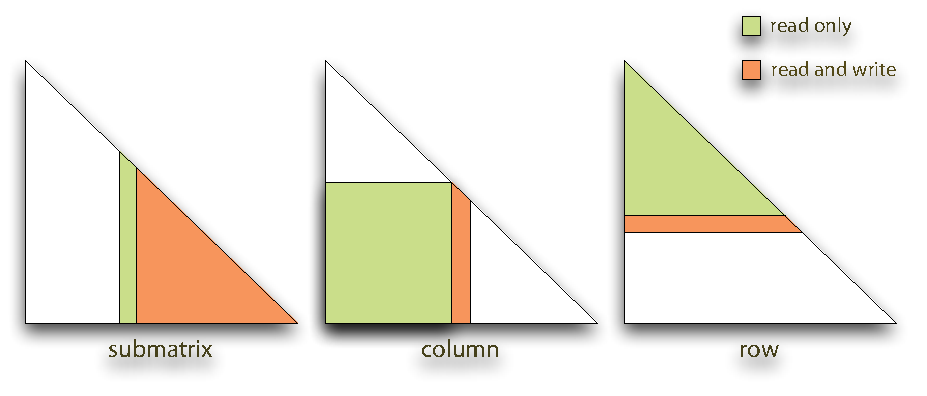
\includegraphics[scale=0.7]{figures/cholesky-memory.pdf}
  \end{figure}
%
\end{frame}

% end of file 
